\documentclass[12pt,letterpaper]{article}
\usepackage[T1]{fontenc}
\usepackage{fullpage}
\usepackage[top=2cm, bottom=4.5cm, left=2.5cm, right=2.5cm]{geometry}
\usepackage{amsmath,amsthm,amsfonts,amssymb,amscd}
\usepackage{lastpage}
\usepackage{enumerate}
\usepackage{fancyhdr}
\usepackage{mathrsfs}
\usepackage{xcolor}
\usepackage{graphicx}
\usepackage{listings}
\usepackage{hyperref}
\usepackage{multirow}
\usepackage{booktabs}
\usepackage[backend=biber,sorting=none]{biblatex}
\usepackage{float}
\addbibresource{references.bib}

\newcommand{\tttilde}[0]{\textasciitilde{}}
\newcommand{\todo}[1]{{\color{blue}{TODO: #1}}}

\newcommand{\authorset}[0]{\mathcal{A}}
\newcommand{\wordset}[0]{\mathcal{W}}

\title{Authorship identification with RNNs}
\author{Nick Fireman}
\date{}

\begin{document}

\maketitle

\section{Introduction}

This project tackles the \emph{authorship identification} problem, which is defined by determining the author of a given passage of text. This is a common application of the field of \emph{stylometry}, which describes the more general attempt to quantify linguistic style in various ways. Authorship identification has clear applications in plagiarism detection, and has also seen use in the fields of law enforcement and intelligence to identify sources of harmful messages.

Early attempts at authorship identification used statistical methods such as principal component analysis to classify texts using human-selected features such as the punctuation frequency or average lengths of words or sentences \cite{binongo1999}. While this has been shown to be effective in certain limited settings, the techniques of deep learning have been found to improve the state-of-the-art performance in more general, realistic, and thus useful contexts. This project shows one such context, where the particularly well-suited recurrent neural network (RNN) architecture is used to classify the authors of public domain literary works.

\section{Approach}

In this project's setting, the possible set of authors $\authorset$ is predetermined and fixed for each experiment, so the authorship identification problem can be viewed as a supervised classification problem, where the network is tasked with mapping an input passage to an author in $\authorset$. As with any other classification problem, the network is trained from a large selection of author-labeled passages for each author in $\authorset$. 

The GloVe model \cite{pennington2014GloVe}  is used to provide a meaningful embedding $G: \wordset \rightarrow \mathbb{R}^n$ of tokens or words $w \in \wordset$ to n-dimensional real-valued vectors. The set $\wordset$ is called the \emph{vocabulary} of the embedding $G$. The vector representations provided by GloVe are designed to respect \emph{analogies}, in the sense that an analogies between two pairs of words $w_1:w_2::w_3:w_4$ (e.g., son : daughter :: father : mother) can be recovered from the words' vector representations. In particular, $|(G(w_2)-G(w_1)) - (G(w_4) - G(w_3))|$ will be small. This can be used to "solve" the analogy for the word $w_4$ (or any other word) by finding the word(s) $w \in \wordset$ minimizing $|G(w_2)-G(w_1) + G(w_3) - G(w)|$. A GloVe embedding is trained via an unsupervised regime, and pretrained embeddings based on various public datasets are used in this project, discussed further in Section \ref{sec:datasets}. 

The process of mapping a substring of an author's work to a list of tokens in $\wordset$ is called \emph{tokenization}, which required some care, since the pretrained GloVe embeddings used in this project have a vocabulary which includes some nonword tokens. In particular, punctuation such as periods, semicolons, and parentheses each have a vector representation in all of the pretrained embeddings, and were split into tokens accordingly. Furthermore, words with apostrophes are also split into two tokens in $\wordset$. For example, $\{\texttt{n't}, \texttt{'re}, \texttt{'ll}\} \subset \wordset$. The tokenizer in the spaCy library \cite{spacy} was used, since it had these tokenization rules implemented by default.

The RNN architecture is used for this project, since it's particularly well-suited for variable-length sequential data such as a list of tokens. To classify a passage with the RNN, the tokens of the passage are input to the RNN one by one, and the final output from the RNN is used to determine the network's classification. Note that the RNN produces an output after each token, but since only the entire passage is being classified, all outputs besides the last one are ignored.

\section{Datasets}
\label{sec:datasets}

\paragraph{Project Gutenberg.} 

Project Gutenberg \cite{gutenberg} is an organization which curates and hosts a collection of literary works in the public domain. These works are made available in many encodings, including UTF-8, which is what this project used. A preprocessed collection of over 3,000 UTF-8 English works written by 142 authors was made publically available by \cite{lahiri:2014:SRW}. The preprocessing specifically involved manual removal of external metadata such as license information and transcribers' notes (i.e. content not written by the original work's author) which is irregularly added to the work's full text by Project Gutenberg. Note that work's metadata written by the original author, such as its table of contents and chapter headings, are left intact in this dataset.

\paragraph{Pretrained GloVe embeddings.}

Alongside introducing the GloVe model, \cite{pennington2014GloVe} also provided datasets of pretrained word vectors, five of which are used in this project. Four pretrained models (400K vocabulary; vectors of dimension 50, 100, 200, and 300, respectively) were built from 6B tokens drawn from Wikipedia and Gigaword 5 (a collection of newswire data). The fifth pretrained model (1.9M vocabulary; vectors of dimension 300) was built from 42B tokens drawn from Common Crawl
\cite{commoncrawl}.

\section{Experiments}

An experiment in this project consists of the following steps:
\begin{itemize}
\item
Training and testing datasets are sampled from the corpus of literature. Each dataset consists of a large number of passages, where each passage contains a fixed number of tokens. The same number of passages are sampled for each author to be classified.

\item 
A pretrained GloVe embedding is used to map each passage to a numeric tensor.

\item 
A number of training iterations are performed, where each iteration trains the RNN model with one hidden layer for 10 epochs using the training dataset, then computes the accuracy of the RNN on the testing dataset. Note that the peak testing accuracy may occur before the last training iteration.

\item
The training loss and the testing accuracy are plotted against the number of epochs trained. This produces a graph that shows how the model improves over the training period. 
\end{itemize}


In this project, the authors Charles Dickens and Mark Twain were classified. Training and testing datasets of 40,000 and 10,000 passages per author were used, respectively, where each passage consists of 30 tokens.
An initial round of $18 = 2 \times 3 \times 3$ experiments were held to find the best configurations of the following three hyperparameters:

\begin{itemize}
    \item The choice of the pretrained GloVe embedding; the \texttt{6B.50d} and \texttt{42B.300d} embeddings were considered.\footnote{ The meaning of e.g. \texttt{6B.50d} is that the model was trained on 6 billion tokens and consists of vectors of dimension 50.}
    \item The size of the RNN's hidden state (referred to as the \emph{hidden size} of the RNN); the sizes 25, 50, and 100 were considered.
    \item The learning rate of the RNN; the rates 0.0005, 0.001, and 0.005 were considered.
\end{itemize}

% Please add the following required packages to your document preamble:
% \usepackage{booktabs}
% \usepackage{multirow}
\begin{table}
\begin{tabular}{@{}|c|c|cccc@{}}
\toprule
\textbf{GLoVE}            & \textbf{Hidden Size} & \textbf{LR}                 & \textbf{Duration (s)}     & \textbf{Peak Test Accuracy}                      & \textbf{Final Acc.}                  \\ \midrule
\multirow{9}{*}{6B.50d}   & \multirow{3}{*}{25}  & \multicolumn{1}{c|}{0.0005} & \multicolumn{1}{c|}{1388} & \multicolumn{1}{c|}{0.7597 (90 epochs)}          & \multicolumn{1}{c|}{0.7586}          \\ \cmidrule(l){3-6} 
                          &                      & \multicolumn{1}{c|}{0.001}  & \multicolumn{1}{c|}{1415} & \multicolumn{1}{c|}{0.7854 (100 epochs)}         & \multicolumn{1}{c|}{0.7854}          \\ \cmidrule(l){3-6} 
                          &                      & \multicolumn{1}{c|}{0.005}  & \multicolumn{1}{c|}{1384} & \multicolumn{1}{c|}{0.7972 (100 epochs)}         & \multicolumn{1}{c|}{0.7972}          \\ \cmidrule(l){2-6} 
                          & \multirow{3}{*}{50}  & \multicolumn{1}{c|}{0.0005} & \multicolumn{1}{c|}{1404} & \multicolumn{1}{c|}{0.7593 (90 epochs)}          & \multicolumn{1}{c|}{0.6640}          \\ \cmidrule(l){3-6} 
                          &                      & \multicolumn{1}{c|}{0.001}  & \multicolumn{1}{c|}{1433} & \multicolumn{1}{c|}{0.7809 (100 epochs)}         & \multicolumn{1}{c|}{0.7809}          \\ \cmidrule(l){3-6} 
                          &                      & \multicolumn{1}{c|}{0.005}  & \multicolumn{1}{c|}{1442} & \multicolumn{1}{c|}{0.7956 (100 epochs)}         & \multicolumn{1}{c|}{0.7956}          \\ \cmidrule(l){2-6} 
                          & \multirow{3}{*}{100} & \multicolumn{1}{c|}{0.0005} & \multicolumn{1}{c|}{1220} & \multicolumn{1}{c|}{0.7631 (100 epochs)}         & \multicolumn{1}{c|}{0.7631}          \\ \cmidrule(l){3-6} 
                          &                      & \multicolumn{1}{c|}{0.001}  & \multicolumn{1}{c|}{1185} & \multicolumn{1}{c|}{0.7897 (100 epochs)}         & \multicolumn{1}{c|}{0.7897}          \\ \cmidrule(l){3-6} 
                          &                      & \multicolumn{1}{c|}{0.005}  & \multicolumn{1}{c|}{1182} & \multicolumn{1}{c|}{0.7947 (90 epochs)}          & \multicolumn{1}{c|}{0.7947}          \\ \midrule
\multirow{9}{*}{42B.300d} & \multirow{3}{*}{25}  & \multicolumn{1}{c|}{0.0005} & \multicolumn{1}{c|}{4710} & \multicolumn{1}{c|}{0.7966 (90 epochs)}          & \multicolumn{1}{c|}{0.7813}          \\ \cmidrule(l){3-6} 
                          &                      & \multicolumn{1}{c|}{0.001}  & \multicolumn{1}{c|}{5191} & \multicolumn{1}{c|}{0.8036 (80 epochs)}          & \multicolumn{1}{c|}{0.7766}          \\ \cmidrule(l){3-6} 
                          &                      & \multicolumn{1}{c|}{0.005}  & \multicolumn{1}{c|}{5320} & \multicolumn{1}{c|}{0.8075 (60 epochs)}          & \multicolumn{1}{c|}{0.7840}          \\ \cmidrule(l){2-6} 
                          & \multirow{3}{*}{50}  & \multicolumn{1}{c|}{0.0005} & \multicolumn{1}{c|}{5439} & \multicolumn{1}{c|}{0.7990 (100 epochs)}         & \multicolumn{1}{c|}{0.7990}          \\ \cmidrule(l){3-6} 
                          &                      & \multicolumn{1}{c|}{0.001}  & \multicolumn{1}{c|}{5332} & \multicolumn{1}{c|}{\textbf{0.8194 (90 epochs)}} & \multicolumn{1}{c|}{0.7929}          \\ \cmidrule(l){3-6} 
                          &                      & \multicolumn{1}{c|}{0.005}  & \multicolumn{1}{c|}{4784} & \multicolumn{1}{c|}{0.7967 (60 epochs)}          & \multicolumn{1}{c|}{0.7810}          \\ \cmidrule(l){2-6} 
                          & \multirow{3}{*}{100} & \multicolumn{1}{c|}{0.0005} & \multicolumn{1}{c|}{4780} & \multicolumn{1}{c|}{0.7959 (90 epochs)}          & \multicolumn{1}{c|}{0.7876}          \\ \cmidrule(l){3-6} 
                          &                      & \multicolumn{1}{c|}{0.001}  & \multicolumn{1}{c|}{4740} & \multicolumn{1}{c|}{0.8083 (90 epochs)}          & \multicolumn{1}{c|}{\textbf{0.8067}} \\ \cmidrule(l){3-6} 
                          &                      & \multicolumn{1}{c|}{0.005}  & \multicolumn{1}{c|}{4701} & \multicolumn{1}{c|}{0.8129 (70 epochs)}          & \multicolumn{1}{c|}{0.7949}          \\ \bottomrule
\end{tabular}
\caption{First round of experimental results.}
\label{tab:results}
\end{table}

The results of this first round of experiments are given in Table \ref{tab:results}. The nine experiments using the \texttt{6B.50d} GloVe model have an average accuracy of $0.7699$, while the same experiments with the \texttt{42B.300d} GloVe model yielded $0.7893$. This shows that a better-trained word embedding model does have a small but noticeable impact on the strength of the resulting RNN. However, comparing the two GloVe models solely by the number of training epochs may be misleading, since the same number of training epochs take roughly four times longer for the larger GloVe model.\footnote{All experiments were performed locally on the same home machine while it was not otherwise in use.}

The highest final accuracy of 0.8067 was attained with the \texttt{42B.300d} model, alongside a hidden size of 100 and a learning rate of 0.001. The highest observed peak accuracy of 0.8194, after 90 epochs of training, was attained from the same learning rate and a hidden size of 50.

The experiments using the \texttt{42B.300d} model fared noticeably worse after the full 100 epochs of training than the \texttt{6B.50d} model. Only one of the experiments using the 300-dimensional GloVe model had a peak accuracy occur after 100 epochs, while only three of the 50-dimensional model experiments peaked in test accuracy before 100 epochs (and those that did peaked at 90, only one iteration before the end of training).

Because of this, a second round of longer experiments was performed using the \texttt{42B.300d} GloVe model, a learning rate of 0.001, and hidden sizes of 50 and 100. These two models were trained three times longer than the first round (for 300 epochs in total) to assess whether the larger GloVe model would do better with more training. 

The results of these experiments is given in Table \ref{tab:round2}, and the test accuracy after each iteration of 10 training epochs is plotted in Figure \ref{fig:acc-round-2}. The dropoff in test accuracy over the last 100 epochs suggests that both models begin to suffer from overfitting at this point. Even so, we find that both models gain some accuracy after the longer training regimen, which suggests that given more time and a larger training dataset, this approach could still yield better results.

% Please add the following required packages to your document preamble:
% \usepackage{booktabs}
% \usepackage{multirow}
\begin{table}
\begin{tabular}{@{}|c|c|c|c|c|c|@{}}
\toprule
\textbf{GLoVe}            & \textbf{Hidden Size} & \textbf{LR}            & \textbf{Duration (s)} & \textbf{Peak Test Accuracy} & \textbf{Final Acc.} \\ \midrule
\multirow{2}{*}{42B.300d} & 50                   & \multirow{2}{*}{0.001} & 15824                 & 0.8289 (170 epochs)         & 0.8188              \\ \cmidrule(lr){2-2} \cmidrule(l){4-6} 
                          & 100                  &                        & 15374                 & 0.8363 (180 epochs)         & 0.8167              \\ \bottomrule
\end{tabular}
\caption{Second round of experimental results.}
\label{tab:round2}
\end{table}

\begin{figure}
    \centering
    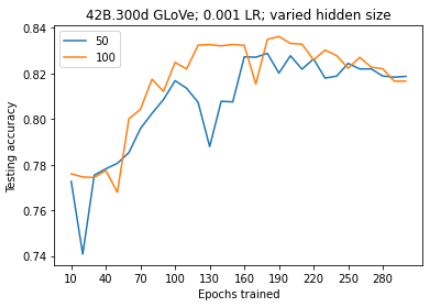
\includegraphics{exp-round-2-.png}
    \caption{Testing accuracy in the second round of experiments.}
    \label{fig:acc-round-2}
\end{figure}

\section{Conclusion}

The above experiments show that the RNN architecture is suitable for authorship identification, showing classification accuracies around 75 to 80\% when distinguishing two authors, which significantly outperforms the expected accuracy of 50\% when randomly guessing. After an initial round of hyperparameter tuning, two promising models were trained for several hours and were shown to achieve nearly 83\% accuracy, though both showed signs of overfitting to the training data. 

The Jupyter nodebook containing the code used to perform all experiments is available on Github\footnote{\url{https://github.com/graftss/authorship-identification/blob/master/authorship-project.ipynb}}. Because the pretrained GloVe word embedding and the collection of books are too large to host on Github, only a small subset of both are hosted in the Github repository. The full pretrained GloVe embeddings are hosted by \cite{glovesite} and the full Project Gutenberg dataset is hosted by \cite{pgdataset}.


\nocite{*}
\printbibliography

\end{document}
